Conforme identificado na elicitação de requisitos, uma das funcionalidades requeridas para a plataforma foi a geração de boletins meteorológicos diários, detalhados anteriormente na Seção \ref{sec:boletim}.

Para que esta funcionalidade fosse implementada adequadamente, um melhor refinamento de sua especificação foi necessário, visando a concepção do mesmo, da linguagem visual a ser adotada e dos elementos que deveriam ser incluídos. Como resultado, obteve-se o modelo apresentado na Figura \ref{fig:modeloBoletim}, que contempla a data, precipitação, temperaturas máxima e mínima, índice de calor, rajada e sua classificação na Escala de Beaufort, e ainda a logomarca do LabInstru e da Universidade do Estado do Amazonas.

\begin{figure}[h!]
	\centering
	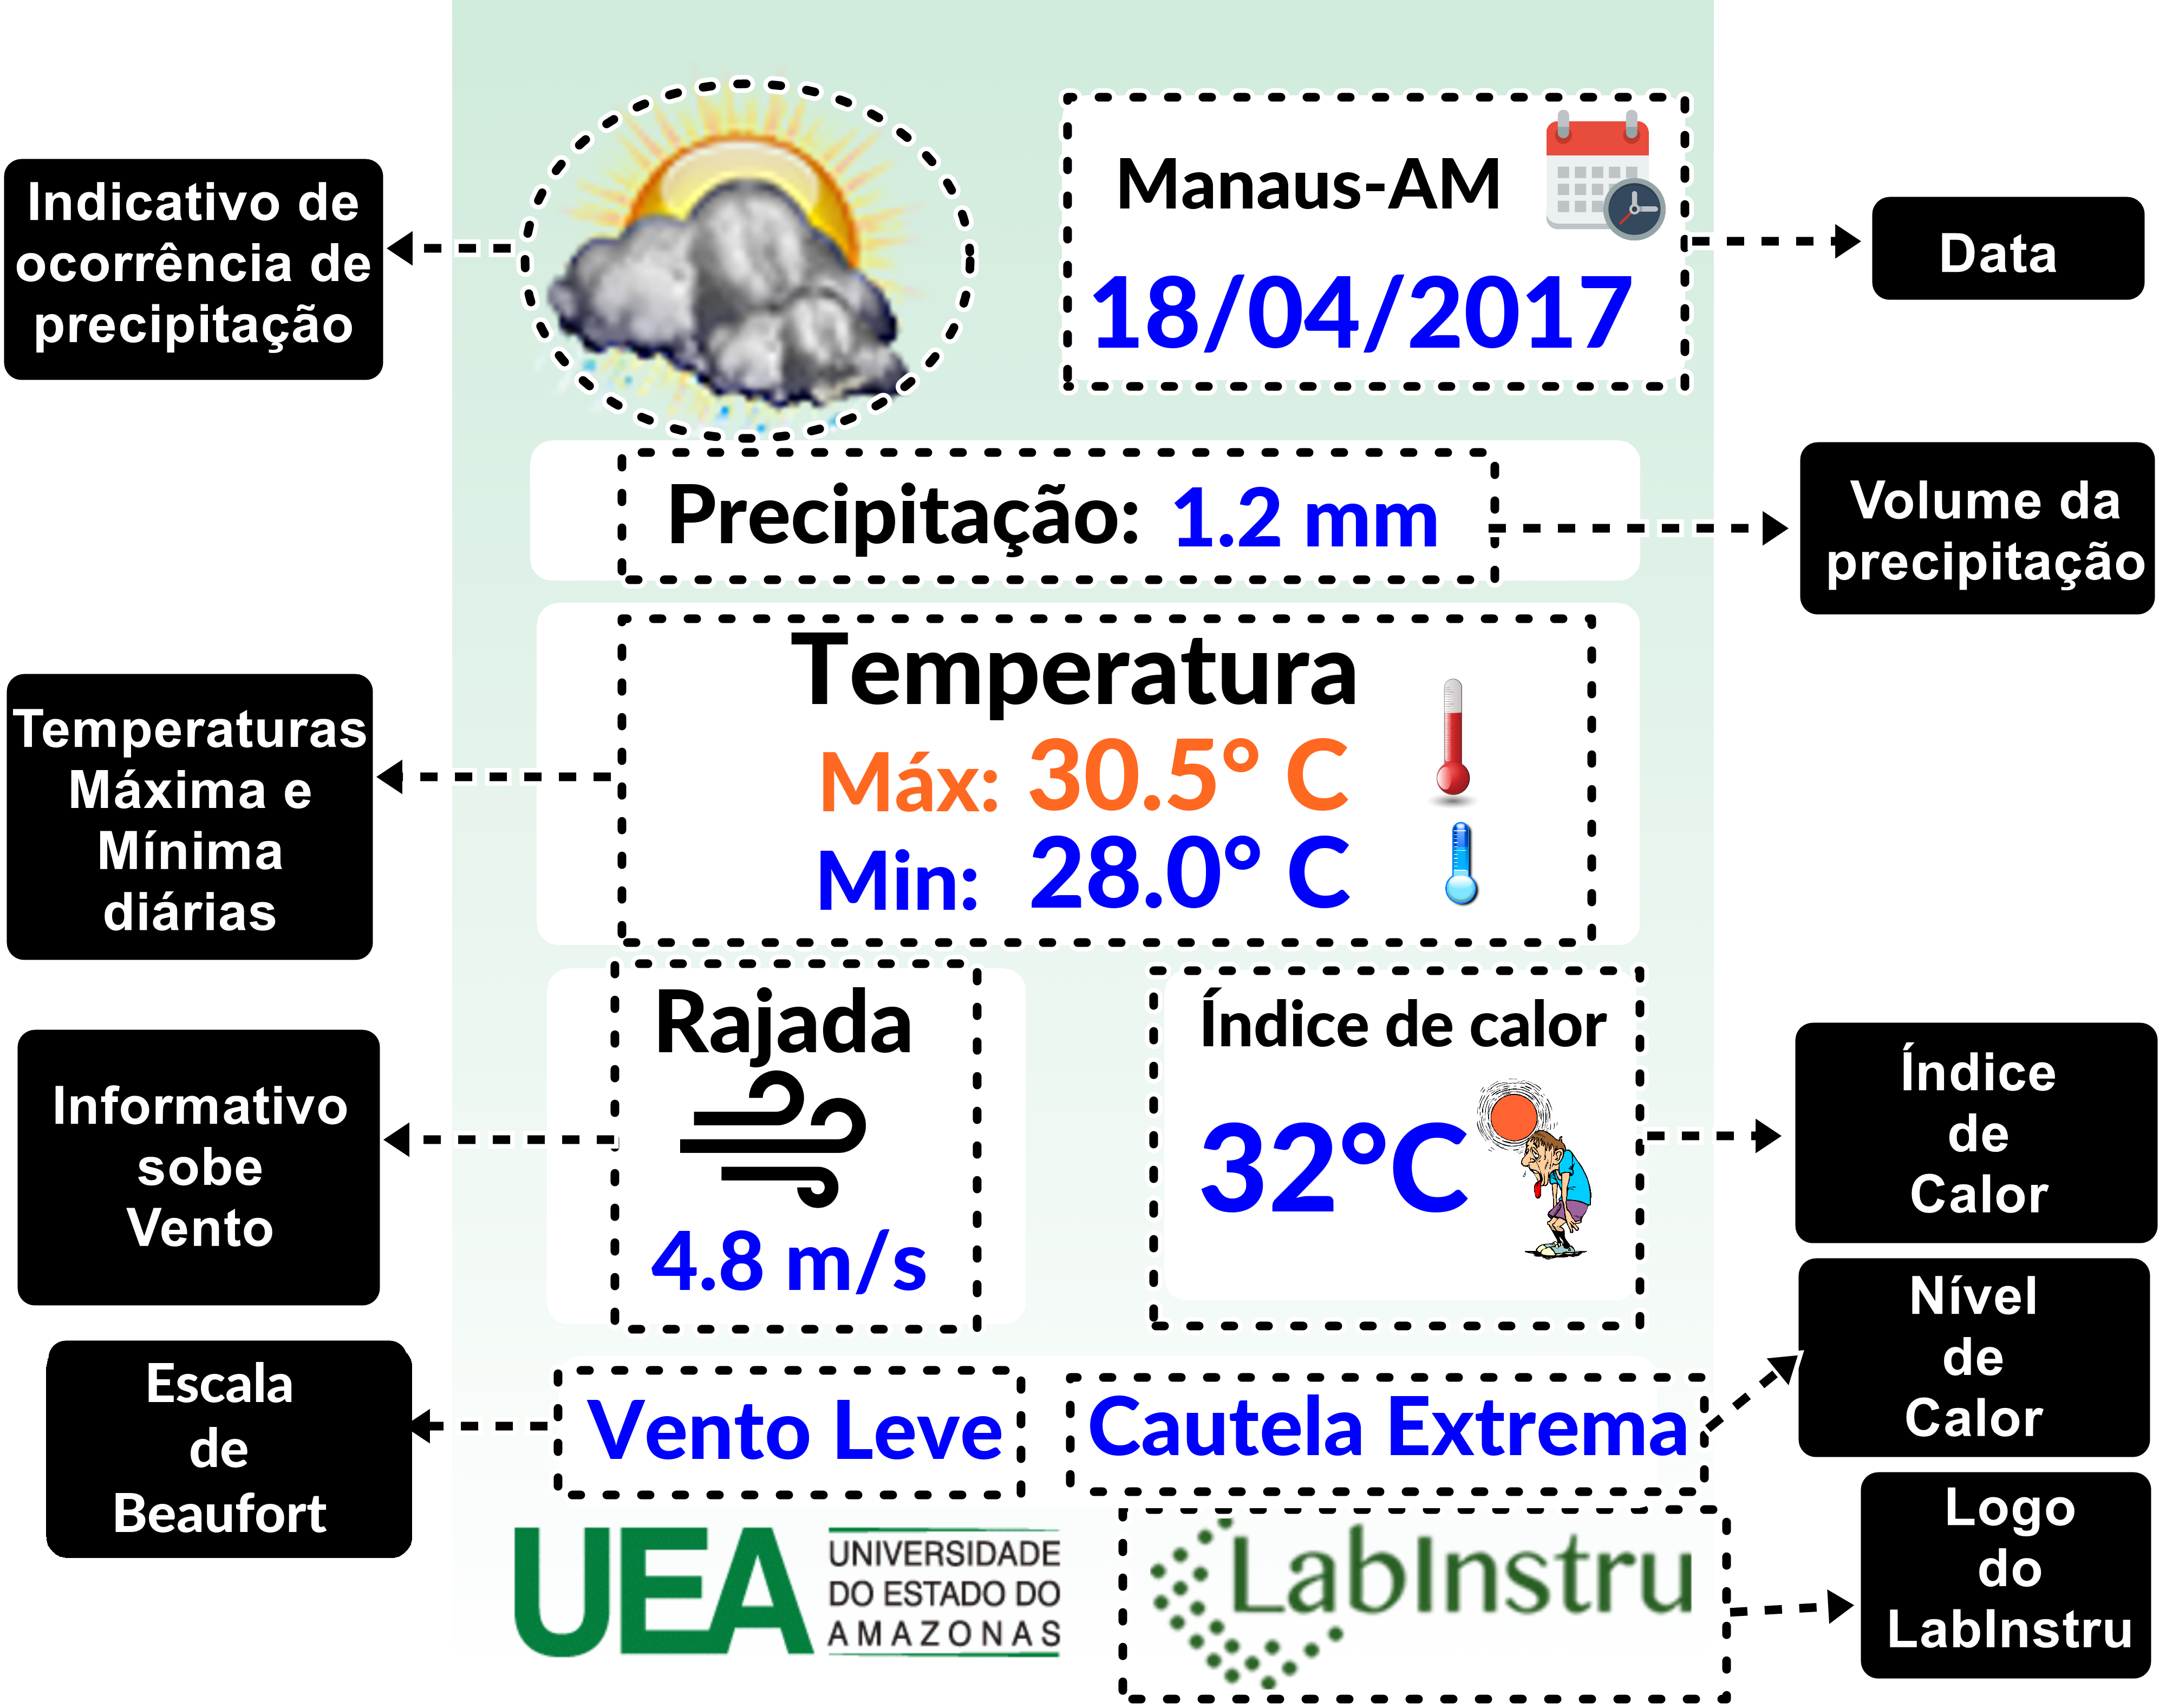
\includegraphics[width=0.5\textwidth]{./img/esbocoBoletim.png}
	\caption{Modelo de referência para boletim meteorológico. Fonte: Próprio autor.} \label{fig:modeloBoletim}
\end{figure}

Para automatizar a geração deste modelo de boletim na solução proposta, foi então necessário implementar o cálculo do índice de calor, desenvolver algoritmos para classificar a rajada e, principalmente, dedicar esforços na interface com o usuário para permitir uma visualização fiel ao modelo discutido com o cliente. Como resultado, o boletim meteorológico produzido com a solução proposta pode ser visto na Figura \ref{fig:boletim}.

\begin{figure}[h!]
	\centering
	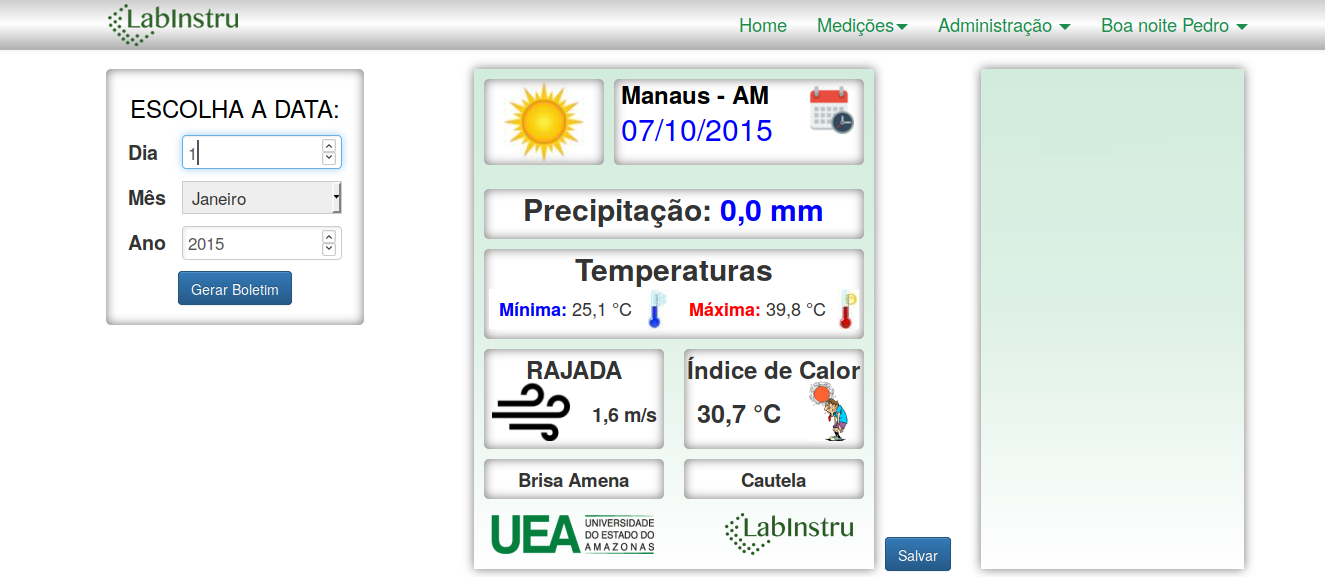
\includegraphics[width=0.9\textwidth]{./img/boletim.png}
	\caption{Boletim meteorológico produzido pelo LabInstru Web. Fonte: Próprio autor.} \label{fig:boletim}
\end{figure}
